% FRAME 1 
\section{Knot}
\begin{frame}{What is a knot}
\centering
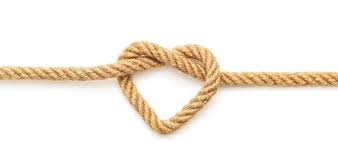
\includegraphics[width=7cm]{Pictures/images.jpg}
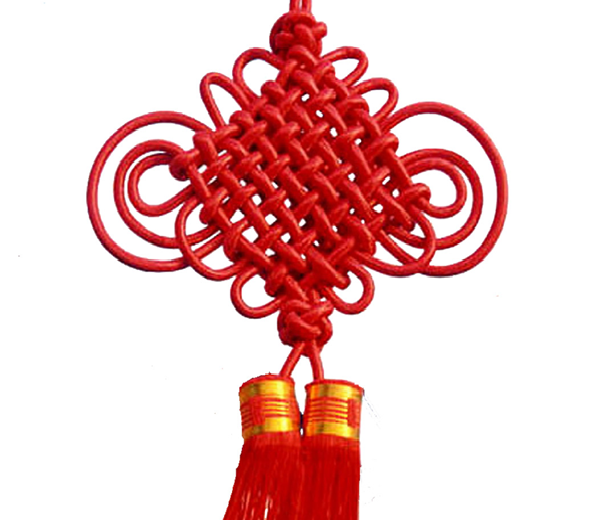
\includegraphics[width=3cm]{Pictures/chineseknot.png}

\end{frame}

% FRAME 2
\begin{frame}{What is a knot}
    \begin{itemize}
        \item Composite knots
    \end{itemize}
\centering
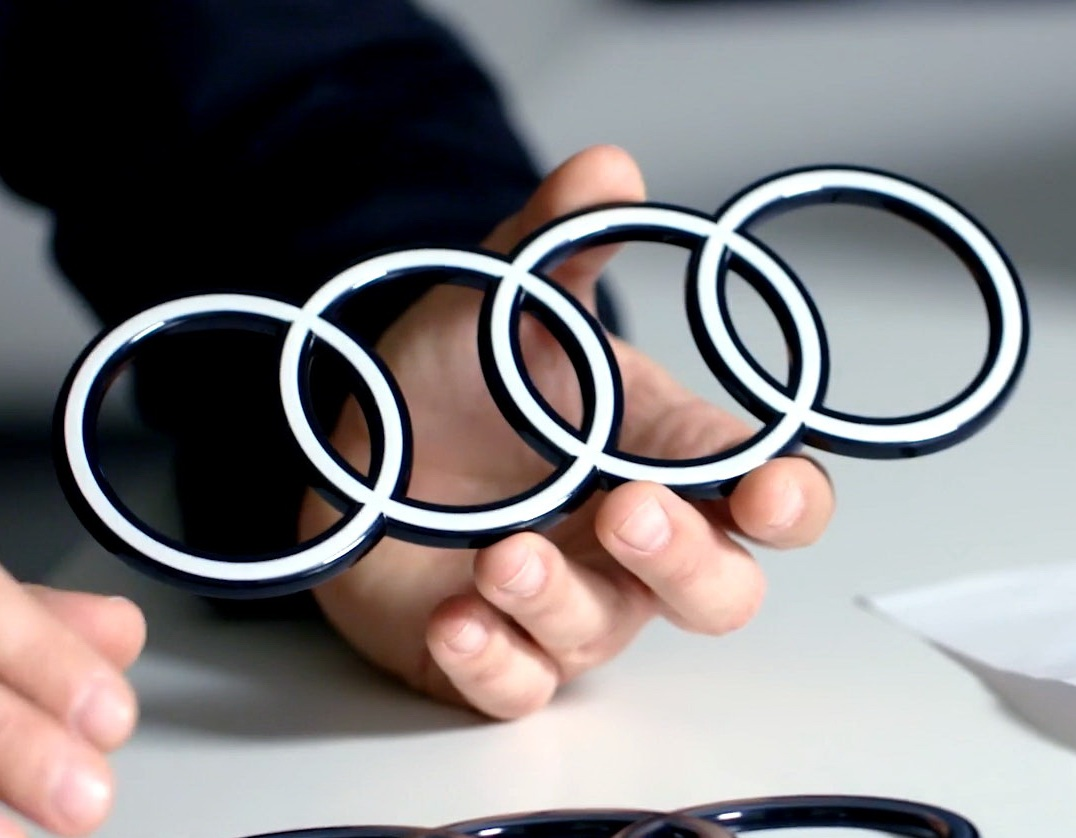
\includegraphics[width = 4.9cm]{Pictures/audi.jpg}
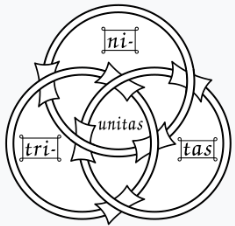
\includegraphics[width = 4cm]{Pictures/borromean.png}

\end{frame}

% FRAME 3 
\begin{frame}{What is a knot}
\begin{itemize}
    \item To study knots rigorously, we need to connect the two ends of the rope.
\end{itemize}
\begin{kulblock}{Definition}
    In mathematics, a knot is an embedding of the circle $\mathbf{S}^1$ into 3-dimensional Euclidean space, $\mathbf{R}^3$.
\end{kulblock}

\end{frame}

% FRAME 4
\begin{frame}{Motivation}
\begin{itemize}
    \item Peter Guthrie Tait and Lord Kelvin (19th century): During the research on composition of atoms, they conjectured that atoms are made out of vortex ring of ether.
\end{itemize}
\centering
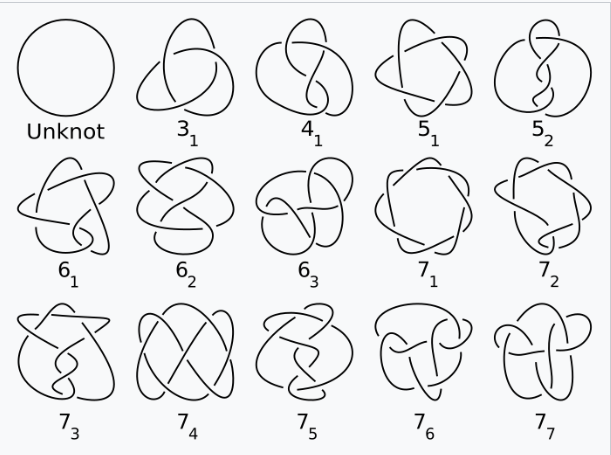
\includegraphics[width=5cm]{Pictures/simple knots.png}
\end{frame}

% FRAME 5
\begin{frame}{Motivation}
\begin{itemize}
    \item The structure of protein and DNA
\end{itemize}
\centering
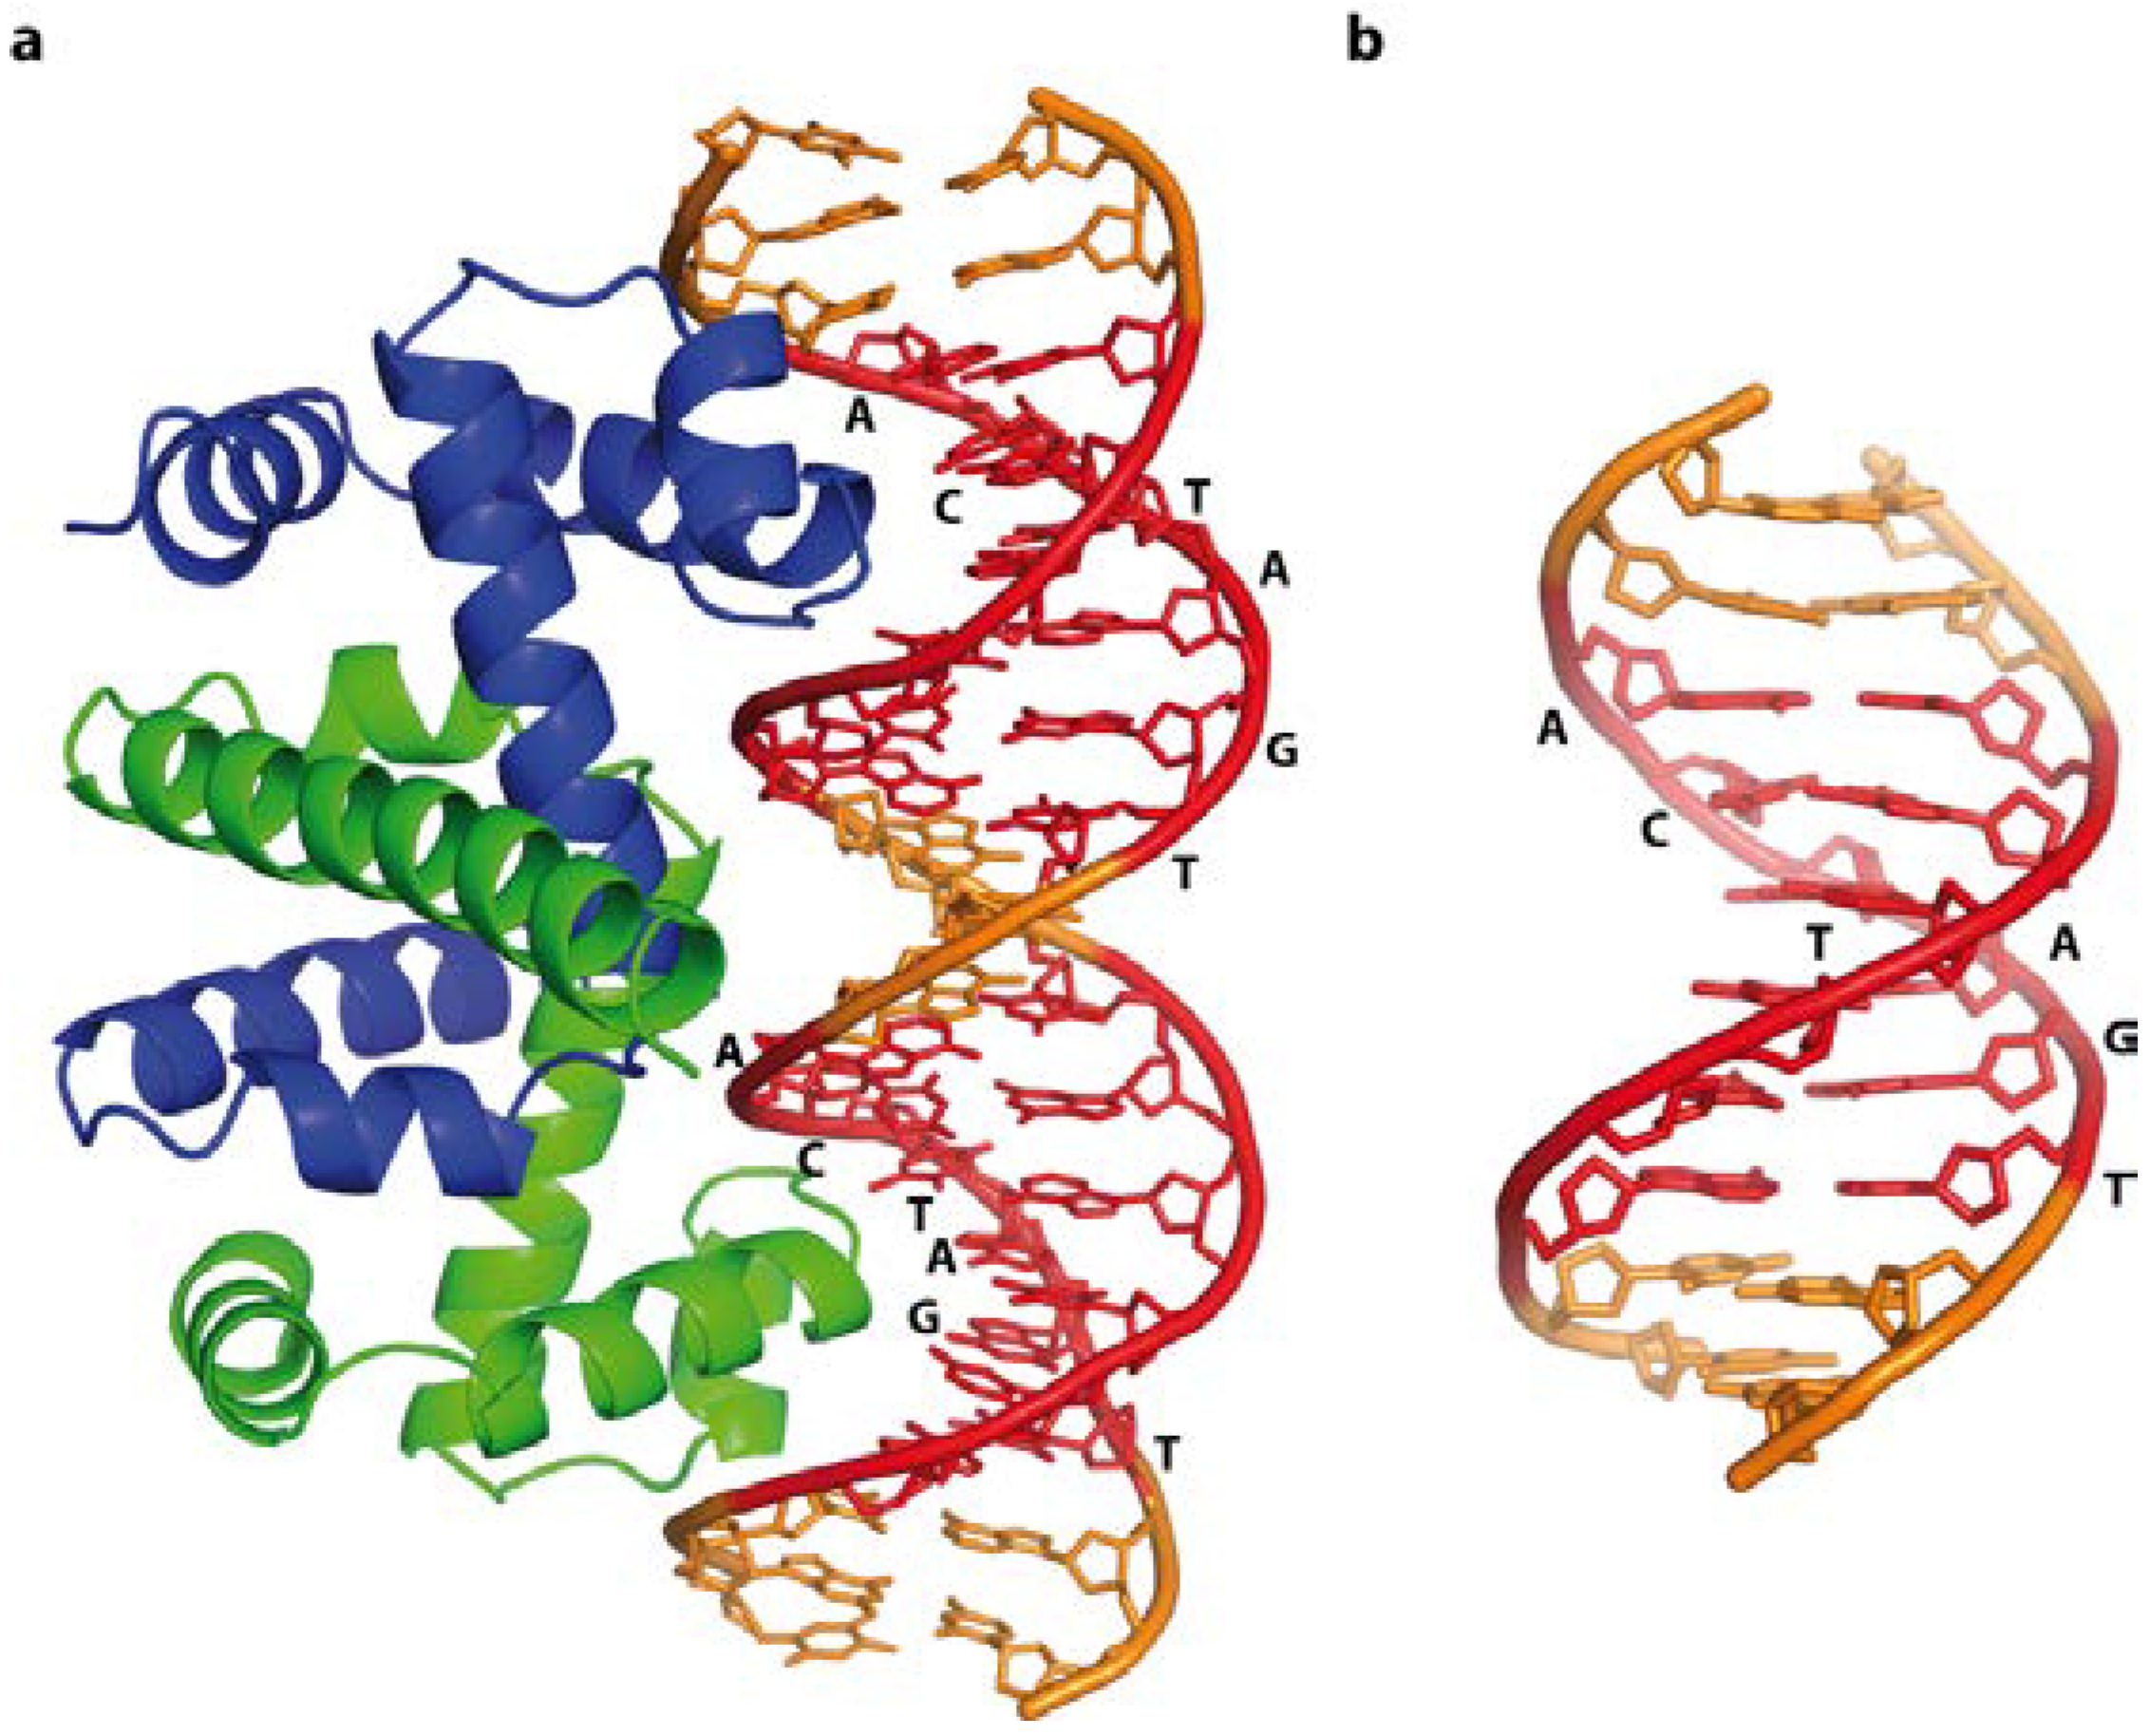
\includegraphics[width=7cm]{Pictures/DNA.png}
\end{frame}

% FRAME 6
\begin{frame}{Motivation}
\begin{itemize}
    \item The knot structure of chemical compound and material
\end{itemize}
\centering
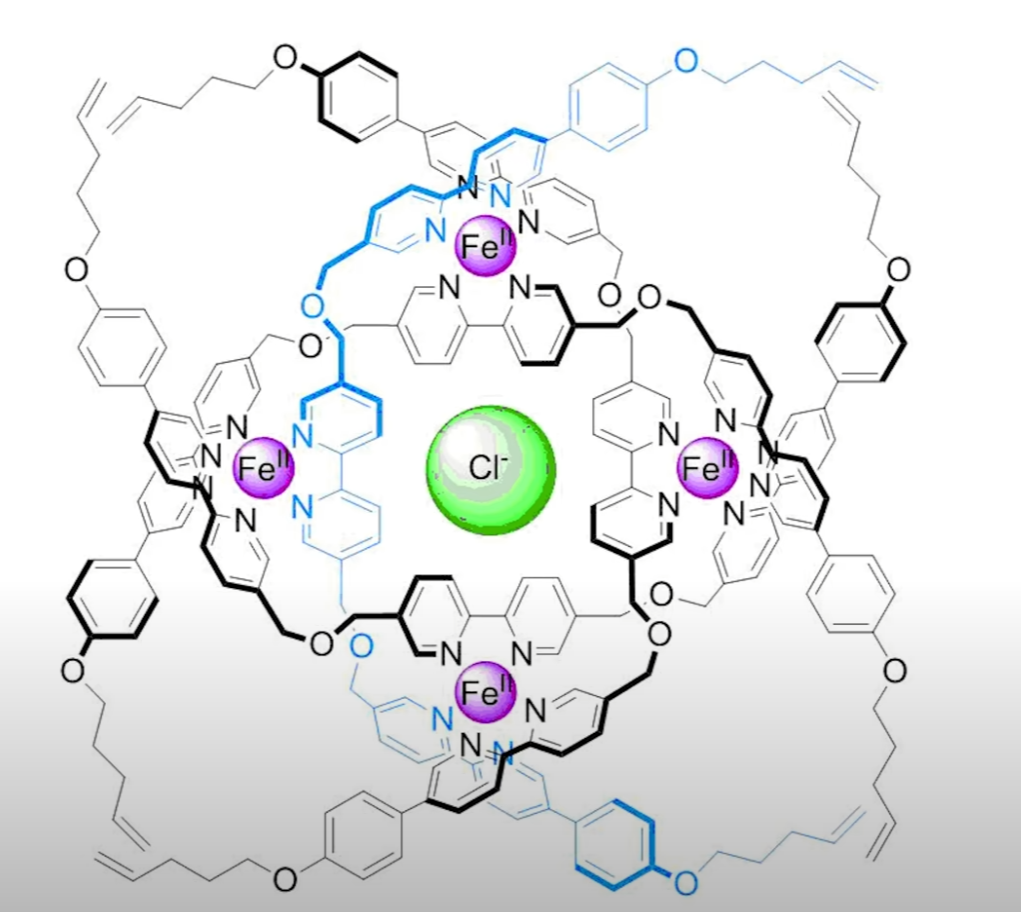
\includegraphics[width = 4.5cm]{Pictures/chemical.png}
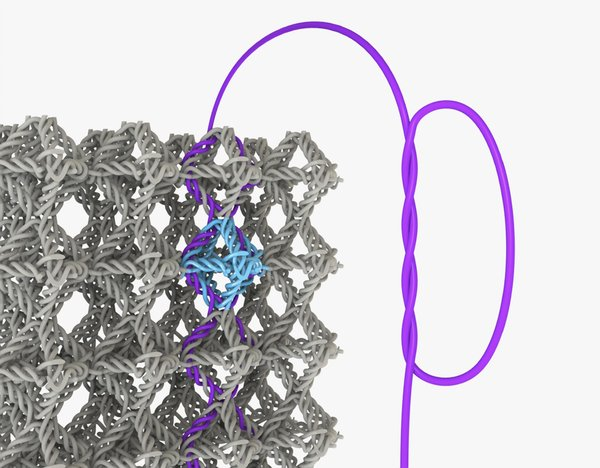
\includegraphics[width=4.5cm]{Pictures/material.jpg}
\end{frame}

% FRAME 7
\begin{frame}{Diagram}
\begin{itemize}
    \item How to represent a knot? Regular projection.
\end{itemize}
\begin{itemize}
    \item A knot projection is called a regular projection if no three points on the knot project to the same point, and no vertex
projects to the same point as any other point on the knot.
\end{itemize}
\end{frame}

% FRAME 8
\begin{frame}{Diagram}

\begin{itemize}
    \item A knot diagram is the regular projection of a knot to the plane with broken
lines indicating where one part of the knot undercrosses the other part.
\end{itemize}
\centering
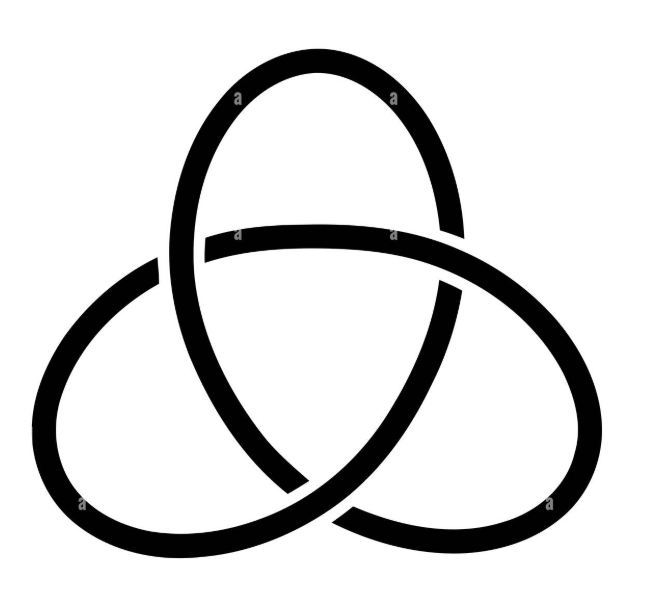
\includegraphics[width=3cm]{Pictures/trefoil.png}
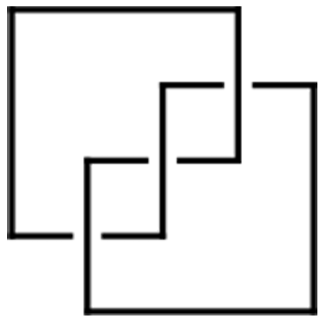
\includegraphics[width=3cm]{Pictures/31.png}
\end{frame}

% FRAME 9
\begin{frame}{Equivalence of knots}
\begin{itemize}
    \item Are they equivalent?
\end{itemize}
\centering
    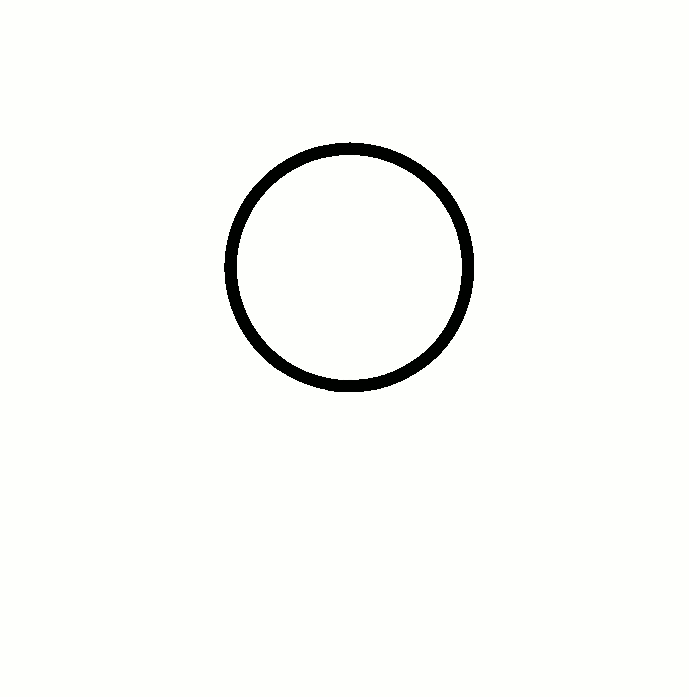
\includegraphics[width = 4cm]{Pictures/Simple.png}
    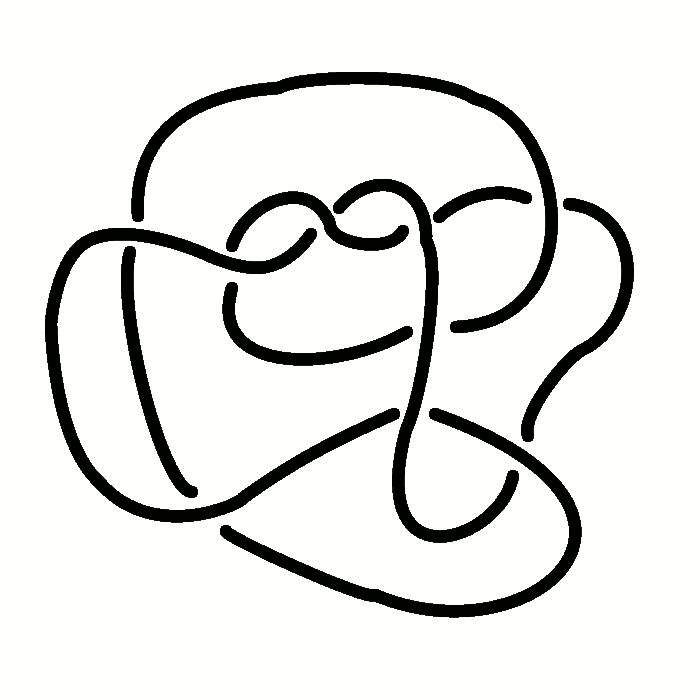
\includegraphics[width = 4cm]{Pictures/complex.png}
\end{frame}


% FRAME 10
\begin{frame}{Reidemeister move}
\begin{itemize}
    \item Equivalence of knot?
\end{itemize}
\centering
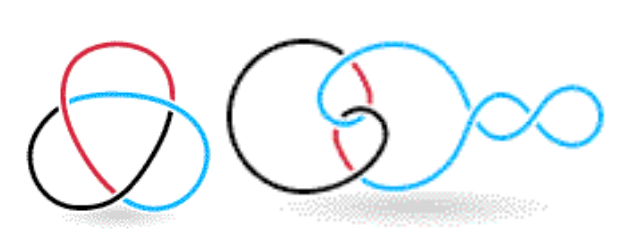
\includegraphics[width=7cm]{Pictures/equivalence.png}

\begin{itemize}
    \item Formal definition: two knots $\mathbf{K}_1$ and $\mathbf{K}_2$ are equivalent if there is an orientation-preserving homeomorphism $h:\mathbb{R}^3 \rightarrow \mathbb{R}^3$ with $h(\mathbf{K}_1) = h(\mathbf{K}_2)$.
\end{itemize}

\begin{itemize}
    \item Reidemeister's Theorem: If two knots are equivalent, their diagrams are related by a sequence of Reidemeister moves.
\end{itemize}
\end{frame}

% FRAME 11
\begin{frame}{Reidemeister move}
\begin{itemize}
    \item A Reidemeister move is an operation that can be performed on the diagram
of a knot whithout altering the corresponding knot.
\end{itemize}
\centering
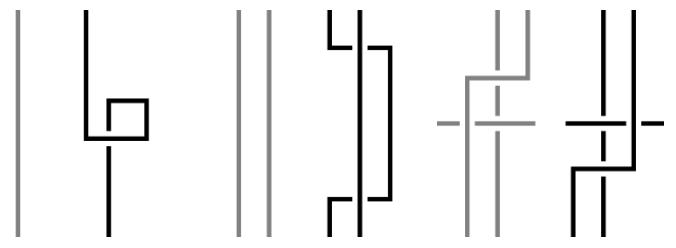
\includegraphics[width=7cm]{Pictures/r.png}
\end{frame}

% FRAME 12
\begin{frame}{Invariant polynomial}
    \begin{itemize}
        \item 1923(James Waddell Alexander): Alexander polynomial $\triangledown$. Reformulated by John Conway in 1969.
\centering
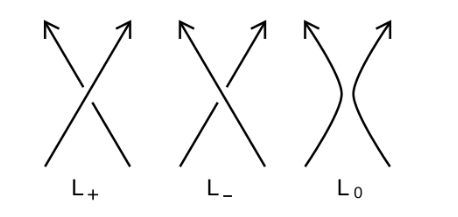
\includegraphics[width =7cm]{Pictures/L.png}
        $$\triangledown(O) = 1$$
        $$\triangledown(L^+) - \triangledown(L^-) = z\triangledown(L_0)$$
    \end{itemize}
\end{frame}

% FRAME 13
\begin{frame}{Invariant polynomial}
\begin{itemize}
    \item 1984(Vaughan Jones): Jones polynomial $V$. Jones won the field's medal for this discovery in 1990.
    $$V(L_0) = 1$$
    $$t^{-1}V(L_+) - tV(L_-) = (t^{\frac{1}{2}} - t^{-\frac{1}{2}})V(L_0)$$
    \item 1985(multiple authors): HOMFLY-PT polynomial $P$: A generalization of the above invariants.
    $$P(L_0) = 1$$
    $$tP(L_+) + t^{-1}P(L_-) + mP(L_0) = 0$$
\end{itemize}
\end{frame}